\chapter{Background}

\section{Definition of terms}

To prevent missunderstandings and confusion, the following subsections 2.1.1 - 2.1.3 will define some terminoligy which will be mandatory for the understanding of certain areas of this thesis.


\subsection{Deep Zoom Image Format}

\begin{figure}[H]
	\begin{center}
		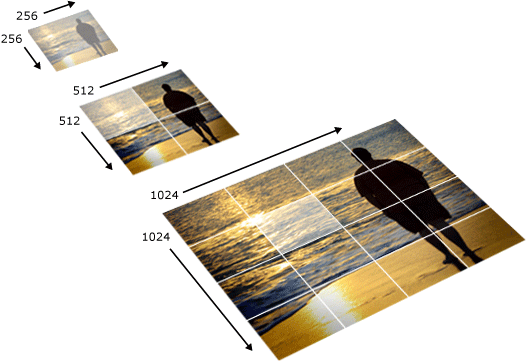
\includegraphics[scale=0.5]{img/dzi_pyramid.png}
		\caption{3 consecutive levels of a dzi image (source: https://i-msdn.sec.s-msft.com/dynimg/IC141135.png)}
		\label{fig:fig2.1}
	\end{center}
\end{figure}

The Deep Zoom Image Format (dzi)\nomenclature{dzi}{Deep Zoom Image Format} is an xml-based file format maintained by Microsoft to improve performance and quality in the handling of large image files. For this purpose an image is represented in a tiled pyramid (see fig. 2.1).

As seen in fig. 2.1 there are multiple versions of a single image in different resolutions. Each resolution in the pyramid is called a \emph{level}. At each level the image is scaled down by the factor 4 (2 in each dimension). Furthermore, the image gets tiled up into $256^2$ tiles (256 in each dimension)\cite{web:dzi}.

If a viewer wants to view a certain area of the image (e.g. the highlighted tile in the last image in fig. 2.1), only the corresponding tiles need to be loaded. This saves large amounts of bandwidth and memory. The same goes for a viewer, who is zoomed out very far. In such a view the full level of detail isn't needed, so that a version from a lower level can be loaded.

A dzi file consists of two parts: a describing .xml file\footnote{Frameworks like \emph{OpenSeaDragon} also support further formats, such as .json.} and a folder with more subfolder. Each subfolder describes a level and as such contains all the tiles for that particular level.


\subsection{Microservice}

The concept of microservices is to seperate one monolithic software construct into several smaller, modular pieces of software. According to \cite{Wolff16}, the idea of microservices is not new, but can be found in the UNIX philosophy. Three basic ideas are stated in \cite{Wolff16}:

\begin{itemize}
	\item A program should fulfill only one task, and it should do it well.
	\item Programs should be able to work together.
	\item Besides, the programs should use a universal interface.
\end{itemize}

As such, microservices are a modularization concept. However, they differ from other concepts, since they are independet from each other. This is a trait, other modularization concepts usually lack. As a result, changes in one microservice don't bring up the necessity of deploying the whole product again but just the one service.

Because of their inherent traits, microservices need to be their own processes in one way or another, may it be as an actual operating system process or as e.g. a docker container\footnote{Docker is a tool, which enables software to be wrapped up in so called "'containers"'. Those containers are a complete, but stripped down, filesystem containing everything the software needs to run (e.g. source code, runtime environment, system tools and libraries, ...). See \url{https://www.docker.com/what-docker}}.

One big advantage of this modularization is that each service can be written in a different programming language, using different frameworks and tools. Furthermore, each microservice can bring along its own support services and data storages, like data bases. It is imperative for the concept of modularization, however, that each microservice has its own storage of which it is in charge of.

A disadvantage of this modularization is, that inter process communication becomes a necessity. However, there are different approaches with which microservices can communicate. \cite{Wolff16} suggests the following:

\begin{itemize}
	\item communication via protocols like REST\footnote{Representational state transfer (REST)\nmc{REST}{Representational state transfer} is architectural style for distributed hypermedia systems, see \cite{Fielding00}.}
	\item an HTML user interfaces with links to other microservices
	\item data replication
\end{itemize}

It is important to define how and with which technology to communicate with, when adressing each microservices to ensure that this particular one can actually be reached with the defined method.


\subsection{Neural Network}
Artificial neural networks (NN)\nmc{NN}{Neural Networks} are a group of models inspiried by biological neural networks\footnote{For the remainder of this thesis, neural network will always represent the artificial one, unless explicitly stated otherwise.}. In a NN, regardless if artificial or biological, many neurons are interconnected with each other. The construct of interconnected neurons can be seperated into layers, of which there are three kinds:

\begin{itemize}
	\item input layer
	\item hidden layer
	\item output layer
\end{itemize}

\begin{figure}[H]
	\begin{center}
		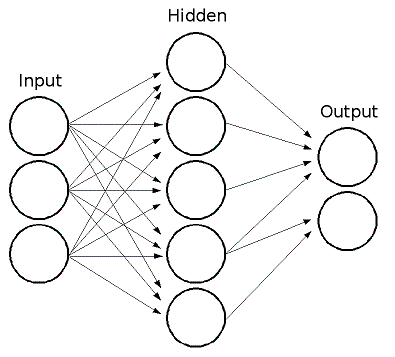
\includegraphics[scale=0.7]{img/mlp.png}
		\caption{3 layer NN (source: http://docs.opencv.org/2.4/\textunderscore images/mlp.png)}
		\label{fig:fig2.2}
	\end{center}
\end{figure}

Basically, the input layer, as the name suggests, is the layer where the NN gets its input data from. After that, there are a number of hidden layers\footnote{A NN doesn't necessarily need to have any hidden layers. For non trivial problems however, it becomes mandatory.}, which are responsible for further computation of the input values. At the end is the output layer which is responsible for communicating the results of the prior operations (compare fig. 2.2). Each single neuron has input values and an output value. Once the input reaches a certain trigger point, the cell in the neuron sends a signal as output. 

A huge benefit of NN, over other software models, is their ability to learn. While certain problems are easier to solve in a sequential, algorithmic fashion (say an equation or the towers of hanoi), certain problems are so complex that new approaches are needed, while other problems can't be solved algorithmic at all. With the use of adequate training samples, a NN can train to solve a problem, not unlike a human, by learning. Since this topic alone is enough for a number of theses, the author refers to \cite{Kriesel07} for further detailed information.


\section{Process Chain}
This section and its following subsections (2.2.1 - 2.2.3) are dedicated to illustrate the process chain necessary to accomplish the research objective stated in chapter 1.2. The process chain consists of the following steps:

\begin{enumerate}[(a)]
	\item convert WHIs of different\footnote{see chap. 2.2.1 for a listing of valid input formats.} formats to dzi format
	\item annotate dzi images with the annotation tool made for this purpose
	\item persist made annotations in a file
	\item seperate annotated images into tiles of custom size
	\item keep correspondence between tiles of an image and its annotations
\end{enumerate}

To fulfill those steps, 3 Microservices will be introduced in the following subsections. Those are:

\begin{itemize}
	\item Conversion Service (see chap. 2.2.1)\\
	This service will be responsible for converting WHIs into the dzi format (a).
	\item Annotation Service (see chap. 2.2.2)\\
	This service will offer a tool to annotate an image (b) and persist made annotations (c).
	\item Tessellation Service (see chap. 2.2.3)\\
	This service will be responsible for seperating an image into tiles (d) and keep the correspondence between tiles and annotations (e).
\end{itemize}


\subsection{Definition of Conversion Service}

The devices which create an WHI, so called whole slide scanners, create images in various formats, depending on the producer. The conversion service has the goal of converting those formats into the dzi format, not only for the purpose of unification, but also to add the deep zoom feature\footnote{See chap. 2.1.1} to the images (see fig. 2.3). This is of special importance, since an average WHI with 1,600 megapixels has a size of approximately 4.6 GB\cite{Farahanil15}.

\begin{figure}[H]
	\begin{center}
		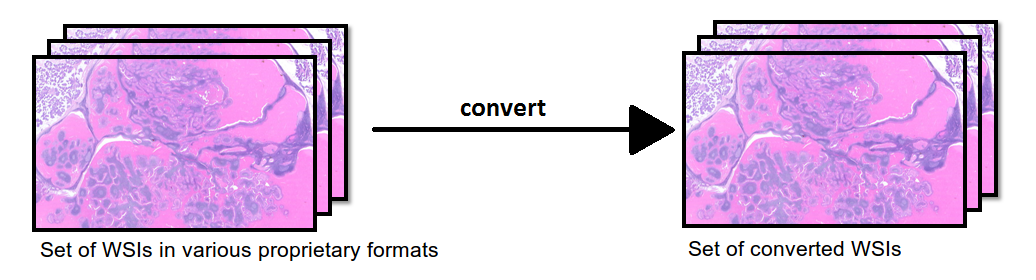
\includegraphics[scale=0.35]{img/processChainA.png}
		\caption{Visualization of the Conversion Service}
		\label{fig:fig2.3}
	\end{center}
\end{figure}

The Conversion Service will be implemented as a python script, which upon calling takes every single WHI of a certain format inside a given folder and converts it to the dzi format. Each converted WHI will be saved in another specified folder. Valid image formats (and their corresponding producers) for conversion are:

\begin{itemize}
	\item .bif (Ventana)
	\item .mrxs (Mirax)
	\item .ndpi (Hamamatsu)
	\item .scn (Leica)
	\item .svs (Aperio)
	\item .svslide (Sakura)
	\item .tif (Aperio, Trestle, Ventana)
	\item .tiff (Philips)
	\item .vms (Hamamatsu)
	\item .vmu (Hamamatsu)
\end{itemize}


\subsection{Definition of Annotation Service}

The first step to create a valid training sample for a NN is to annotate the WHIs which will later serve as that. To do so, a GUI\nmc{GUI}{Graphical User Interface} must be deployed which enables a pathologist to make annotations to an WHI. Additionally, the Annotation Service also needs to be capable to persist made annotations (see fig. 2.4). This will happen by saving the annotations into a file which will be placed next to the image.

\begin{figure}[H]
	\begin{center}
		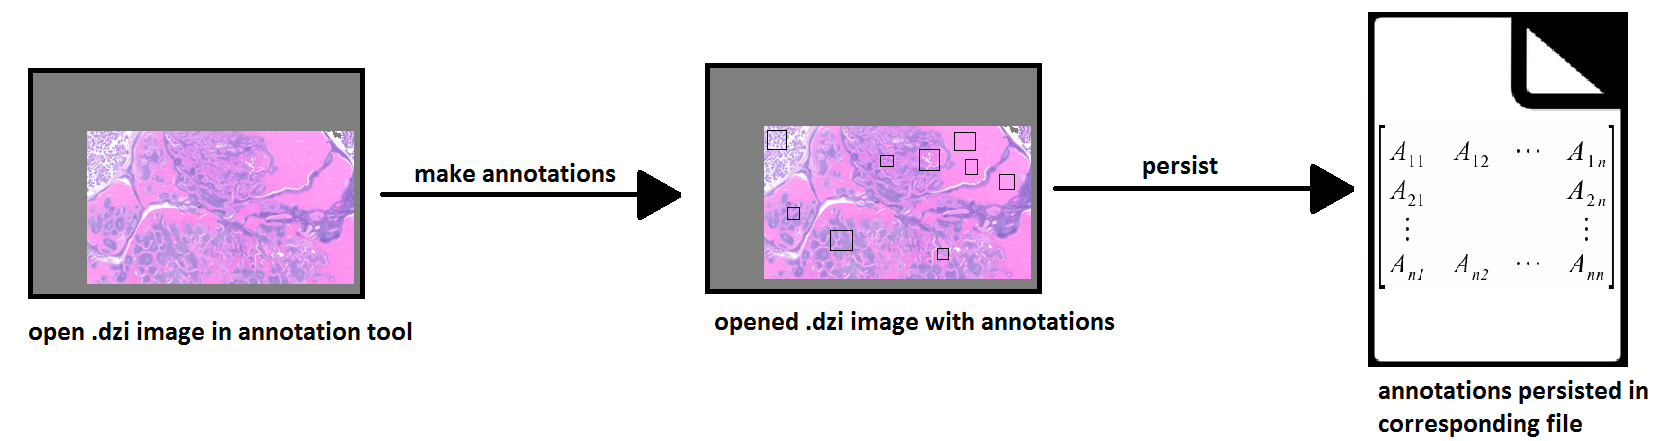
\includegraphics[scale=0.25]{img/processChainB.png}
		\caption{Visualization of the Annotation Service}
		\label{fig:fig2.4}
	\end{center}
\end{figure}

To enable the pathologist to make annotations in the first place, a GUI needs to be offered by the service. This GUI will be developed in iterations with the help of a number of pathologists to adapt it to their wishes and grant the best possible usability. The basic concept of the first iteration will be based on the Microdraw\footnote{See \url{https://github.com/r03ert0/microdraw} for more information on the Microdraw project} GUI (see fig. 2.5).

\begin{figure}[H]
	\begin{center}
		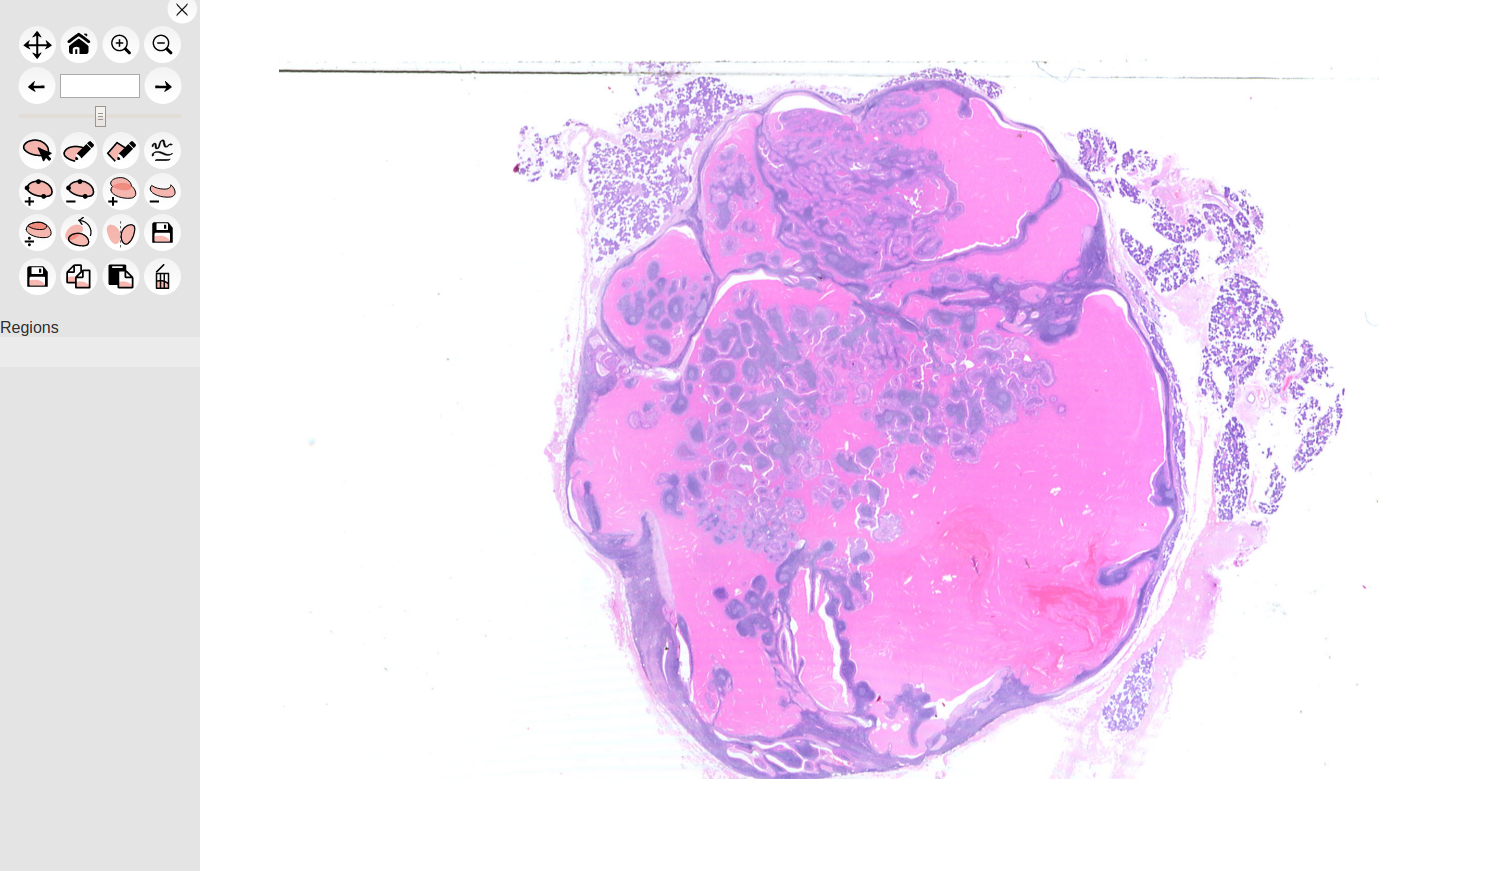
\includegraphics[scale=0.2]{img/microdrawUI.png}
		\caption{Microdraw GUI with opened WHI}
		\label{fig:fig2.5}
	\end{center}
\end{figure}

Microdraw is a webbased annotation tool, which describes itself as

\begin{quotation}
"(...) a collaborative vectorial annotation tool for ultra high resolution data, such as that produced by high-throughput histology." \cite{web:microdraw}
\end{quotation}

Therefore, the GUI of the Annotation Service, or Annotation Service Viewer (ASV)\nmc{ASV}{Annotation Service Viewer}, will run as a web application in a browser. Annotations will be made by selecting a shape or annotation method from the various tools in the toolbar (see the gray bar on the left in fig. 2.5). After selecting the area to be annotated, an actual description of that area can be made via keyboard input.

When the pathologist is done or wants to save the made annotations, the Annotation Service will create a file in which they will be persisted in. Only one WHI can be opened in one ASV at a time.


\subsection{Definition of Tessellation Service}

The task of the Tessellation Service is to tessellate a given WHI into multiple tiles while keeping up the correspondence between image areas and annotations (see fig. 2.6). Tessellation describes the process of seperating a geometric space (e.g. a plane) into multiple tiles of one or more shapes. No matter if the tiles are unifrom or of different shapes, there must be no gaps or overlapping areas in the resulting tiles.

\begin{figure}[H]
	\begin{center}
		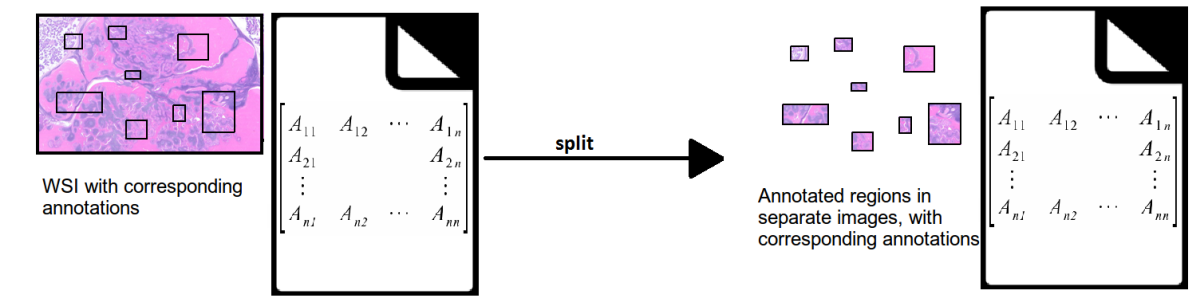
\includegraphics[scale=0.3]{img/processChainC.png}
		\caption{Visualization of the Tessellation Service}
		\label{fig:fig2.6}
	\end{center}
\end{figure}

The tessellation of the Tessellation Service differs from the given definition in two aspects. First, all tiles will be of a unifrom shape (square). Second, the service will also offer the possibility of seperating only the annotated areas of an WHI into tiles. Therefore, the "no gaps" rule is invalid, when this option is chosen. The rule of no overlapping areas holds true in either case, however.

As mentioned before, the second task of the Tessellation Service is to ensure the correspondence between tiles and annotations of the original WHI. This means that, if the original WHI has an annotation in the area of a tile, this tile needs to have the same annotation.
